% ========================================
% Chapitre 1 : Présentation du problème
% ========================================
\chapter{Présentation du problème}

\section*{Références principales}
\[
\begin{cases}
\text{Mathematics of Arbitrage (Schachermayer \& Delbaen), Chapitre 2},\\[3pt]
\text{Introduction to Stochastic Calculus (Lamberton \& Lapeyre), Chapitres 1 et 2.}
\end{cases}
\]

\section{Le modèle}

\begin{definition}[Temps discret fini]
Le temps est modélisé par un ensemble discret fini :
\begin{equation}
t \in \{0, 1, \ldots, T\}.
\end{equation}
\end{definition}

\begin{definition}[Espace probabilisé]
On considère un espace probabilisé $(\Omega, \mathcal{F}^{P}, P)$ avec $\Omega$ fini, $\mathcal{F}^{P} = \mathcal{P}(\Omega)$ et $\forall \omega \in \Omega,\; P(\omega)>0$. On a $\text{card}(\mathcal{P}(\Omega)) = 2^n$ et $\text{card}(\Omega) = n$.
\end{definition}

\medskip
\begin{tcolorbox}[title=Interprétation intuitive, colback=yellow!5!white, colframe=yellow!50!black]
\begin{itemize}
    \item $\Omega$ : espace des configurations économiques possibles sur $[0,T]$ ;
    \item $\mathcal{F}^{P}$ : information disponible sur la période ;
    \item $P$ : probabilité historique.
\end{itemize}
\end{tcolorbox}

\begin{definition}[Filtration]
L'information est modélisée par une filtration $\mathcal{J}^{P} = (\mathcal{J}^{P}_{t})_{t=0,\ldots,T}$ définie par :
\begin{equation}
\mathcal{J}^{P} = (\mathcal{J}^{P}_{t})_{t=0,\ldots,T}, \quad \mathcal{J}^{P}_{0}=\{\emptyset,\Omega\}, \quad \mathcal{J}^{P}_{T}=\mathcal{F}^{P}.
\end{equation}
où $\mathcal{J}^{P}_{0}$ est la plus petite $\sigma$-algèbre.
\end{definition}

\begin{definition}[Actifs financiers]
Le marché est composé de $d+1$ actifs financiers :
\begin{enumerate}
    \item \textbf{Actif sans risque} (numéraire) : $(S_t^0)_{t=0,\ldots,T}$ adapté à $(\mathcal{J}_t)$, avec $S_t^0(\omega)>0$.
    \begin{equation}
    (S_t^0)_{t=0,\ldots,T} \text{ adapté à } (\mathcal{J}_t), \quad S_t^0(\omega)>0.
    \end{equation}
    
    \item \textbf{Actifs risqués} : $d \in \mathbb{N}^*$ actifs. La valeur à la date $t$ de l'actif $j$ est notée $S_t^j$.
    \begin{equation}
    S_t = (S_t^0, S_t^1, \ldots, S_t^d).
    \end{equation}
\end{enumerate}
\end{definition}

\begin{remarques}
\item L'hypothèse $\Omega$ fini est essentielle : les espaces $L^0,L^p,L^\infty$ sont isomorphes à $\RR^{|\Omega|}$.
\item L'actif sans risque joue le rôle de numéraire : $S_t^0 = e^{rt}$.
\item Variable aléatoire mesurable :

$X : (\Omega, \mathcal{A}) \longrightarrow (\mathbb{R}, \mathcal{B}(\mathbb{R}))$

$X \text{ variable aléatoire mesurable} \Longleftrightarrow \forall B \in \mathcal{B}(\mathbb{R}), \; X^{-1}(B) \in \mathcal{A}$

$P_X : \mathcal{B}(\mathbb{R}) \longrightarrow [0,1], \quad B \longmapsto P(X^{-1}(B))$

\vspace{1em}
\textbf{Si } $\mathcal{A} = \{\emptyset, \Omega\}$, 
alors $X$ variable aléatoire $\Longleftrightarrow X$ constante.

\vspace{1em}

\textbf{Si } $\mathcal{A} = \mathcal{F}_t = \mathcal{P}(\Omega)$

\text{Quel est le sens d'être } $\mathcal{F}_t$-mesurable ? Une variable aléatoire dans ce cas est simplement une application.

\vspace{1em}
\item Mesurabilité :
$\hat{S}_{t+1}$ est $\mathcal{F}_{t+1}$-mesurable mais pas $\mathcal{F}_t$-mesurable. $\Rightarrow$ On peut être dans $\mathcal{F}_{t+1}$ sans être dans $\mathcal{F}_t$

\end{remarques}

\section{Processus adapté à une filtration}

\begin{tcolorbox}[title=Intuition générale, colback=green!5!white, colframe=green!50!black]
Un processus stochastique $(X_t)_{t=0,\dots,T}$ est dit \textbf{adapté} à une filtration $(\mathcal{F}_t)_{t=0,\dots,T}$ si, à chaque instant $t$, 
la variable aléatoire $X_t$ est \textbf{connue à ce moment-là}, c'est-à-dire \textbf{mesurable} par rapport à $\mathcal{F}_t$.

\medskip
Autrement dit :
\begin{center}
\textbf{Être adapté} $\Longleftrightarrow$ $X_t$ dépend uniquement de l'information disponible jusqu'au temps $t$.
\end{center}
\end{tcolorbox}

\begin{definition}[Définition formelle]
Un processus $(X_t)_{t=0,\dots,T}$ est \textbf{adapté} à la filtration $(\mathcal{F}_t)$ si :
\[
\forall t \in \{0,1,\dots,T\}, \quad X_t \text{ est } \mathcal{F}_t\text{-mesurable.}
\]
Autrement dit :
\[
\forall B \in \mathcal{B}(\mathbb{R}), \quad X_t^{-1}(B) \in \mathcal{F}_t.
\]
\end{definition}

\paragraph*{Interprétation et Importance de l'Adaptation}
La condition qu'un processus de prix $(S_t)$ soit "adapté" à une filtration $(\mathcal{F}_t)$ est une formalisation mathématique d'une idée fondamentale et intuitive : on ne peut pas connaître le futur. Une analogie simple est celle d'un jeu de cartes : à chaque tour $t$, la filtration $\mathcal{F}_t$ représente l'ensemble des cartes que vous avez vues jusqu'à présent. Une stratégie "adaptée" signifie que votre décision de mise au tour $t$ ne peut dépendre que de ces cartes visibles, et non des cartes encore dans le paquet. En finance, cela signifie que la valeur d'un actif $S_t$ à l'instant $t$ est une information connue à cet instant, déterminée par l'historique des événements du marché jusqu'à $t$, mais que sa valeur future $S_{t+1}$ reste incertaine.


\begin{exemple} [Interprétation économique]
En finance, $\mathcal{F}_t$ représente \textbf{l'information disponible sur le marché} au temps $t$.
Dire que le prix d'un actif $S_t$ est $\mathcal{F}_t$-mesurable signifie que sa valeur est \textbf{connue à la date $t$}
à partir des informations de marché.

Ainsi, un processus de prix $(S_t)$ \textbf{adapté} signifie que :
\[
S_t \text{ dépend du passé et du présent, mais pas du futur (on ne connaît pas } S_{t+1} \text{ à la date } t).
\]
\end{exemple}



\section{Actifs risqués et actif sans risque ; rappel sur $L^p$ (cas $\Omega$ fini)}

\begin{definition}[Actifs risqués]
Soit $d\in\mathbb{N}^*$ le nombre d'actifs risqués. Pour tout $j\in\{1,\dots,d\}$ et
$t\in\{0,\dots,T\}$, on note
\begin{equation}
\hat S_t^{\,j}\quad\text{la valeur à la date }t\text{ du $j$-ième actif risqué.}
\end{equation}
On suppose que, pour tout $j$, le processus $\big(\hat S_t^{\,j}\big)_{t=0,\dots,T}$ est adapté à la
filtration $\big(\mathcal{J}_t\big)_{t=0,\dots,T}$. \emph{Remarque.} Contrairement à l'actif sans risque,
un actif risqué peut (en principe) toucher $0$.
\end{definition}

\begin{definition}[Notation vectorielle]
On regroupe les prix en un vecteur
\begin{equation}
\hat S_t:=\big(\hat S_t^{\,0},\hat S_t^{\,1},\dots,\hat S_t^{\,d}\big)\in\RR_+^{\,d+1},
\end{equation}
de sorte que $\hat S=(\hat S_t)_{t=0,\dots,T}$ est un processus stochastique à valeurs dans $\RR^{d+1}$, adapté à
$(\mathcal{J}_t)$.
\end{definition}

\begin{definition}[Actif sans risque et numéraire]
L'actif non risqué (compte monétaire) joue le rôle de numéraire. Dans les modèles élémentaires
(et dans cette partie du cours), on suppose qu'il est possible d'emprunter/prêter au taux
constant $r>0$ \emph{en composition continue}. On pose alors
\begin{equation}
\hat S_t^{\,0}=e^{rt},\qquad t\in\{0,\dots,T\},
\end{equation}
c'est-à-dire la valeur à la date $t$ d'un euro placé à la date $0$.
\end{definition}

\bigskip
\paragraph{Remarques techniques (cas $\Omega$ fini).}
Pour des raisons d'analyse fonctionnelle, on supposera $\Omega$ \emph{fini}. En particulier,
les espaces
\[
L^0(\Omega,\mathcal{F},P),\quad L^p(\Omega,\mathcal{F},P)\ (1\le p<\infty),\quad
L^\infty(\Omega,\mathcal{F},P)
\]
s'identifient tous canoniquement à $\RR^{|\Omega|}$ (donc une seule topologie « naturelle »).
On rappelle les définitions usuelles :
\[
\begin{aligned}
L^0(\Omega,\mathcal{F},P)
&=\bigl\{\,X:\Omega\to\RR\ \bigm|\ X\ \text{est }\mathcal{F}\text{-mesurable}\,\bigr\},\\[2mm]
L^p(\Omega,\mathcal{F},P)
&=\Bigl\{\,X\in L^0\ \Bigm|\ \E\bigl[|X|^p\bigr]<\infty\Bigr\},
\quad 1\le p<\infty,\\[2mm]
L^\infty(\Omega,\mathcal{F},P)
&=\Bigl\{\,X\in L^0\ \Bigm|\ \exists M>0\ \text{tel que }P(|X|\le M)=1\Bigr\}.
\end{aligned}
\]
Quand $\Omega$ est fini, toutes les normes usuelles sont équivalentes et
\(
L^0\simeq L^p\simeq L^\infty\simeq \RR^{|\Omega|}.
\)


\subsubsection*{Convention sur les taux d'intérêt}

La modélisation de l'actif sans risque est une pierre angulaire de la théorie financière. Il sert de numéraire, c'est-à-dire d'étalon de valeur permettant de comparer des flux monétaires à différentes dates. Le choix de sa dynamique est donc crucial. En pratique, la valeur future d'un capital dépend de la fréquence de composition des intérêts. Le tableau suivant illustre les différentes conventions et justifie le choix de la composition continue, $S^0_t = e^{rt}$, qui offre une simplification mathématique et une représentation idéalisée d'un marché financier sans friction.

\begin{center}
\begin{tabular}{l|lll}
\textbf{Composition} & \textbf{Valeur à $t=1$} & \textbf{Valeur à $t=T$} \\
\hline
Annuelle & $(1 + r)$ & $(1 + r)^T$ \\
Semestrielle & $(1 + r/2)^2$ & $(1 + r/2)^{2T}$ \\
Journalière & $(1 + r/365)^{365}$ & $(1 + r/365)^{365T}$ \\
$m$ périodes/an & $(1 + r/m)^m$ & $(1 + r/m)^{mT}$ \\
\textbf{Continue ($m \to +\infty$)} & \boldmath{$e^r$} & \boldmath{$e^{rT}$} \\
\end{tabular}
\end{center}

C'est cette convention (composition continue) que nous retiendrons pour la suite : $S^0_t = e^{rt}$.

\section{Binomial Model ($T=3$, $d=1$)}

\subsubsection*{NON RISKY}
$S_0^0 = e^{rt}$

\subsubsection*{RISKY}
$P(w_1, w_2) = P(w_2 \mid w_1) \cdot P(w_1)$

$P(w_1) = \begin{cases}
P(u) \\
P(d)
\end{cases}$

\vspace{1cm}

\begin{center}
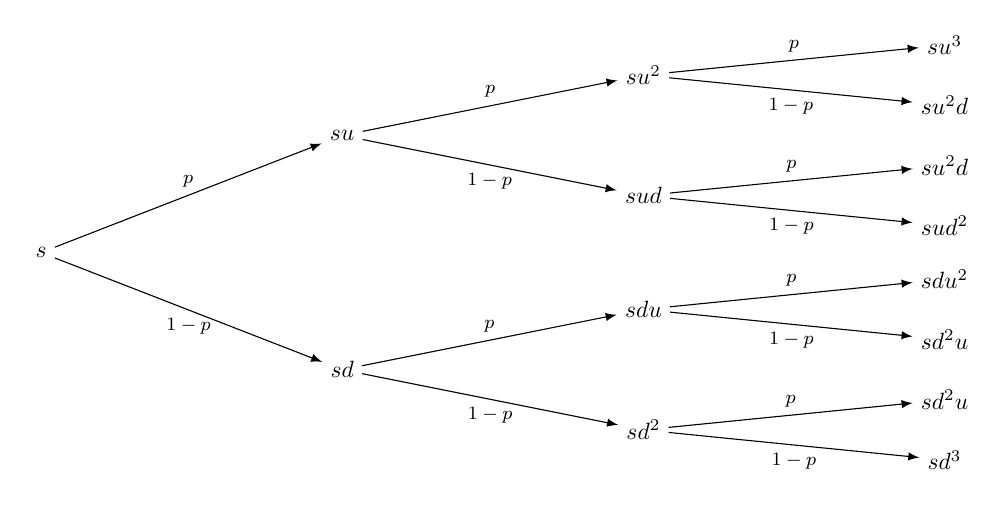
\begin{tikzpicture}[
    grow=right,
    scale=0.85, transform shape,
    level distance=45mm,
    level 1/.style={sibling distance=35mm},
    level 2/.style={sibling distance=18mm},
    level 3/.style={sibling distance=9mm},
    edge from parent/.style={draw, -latex},
    every node/.style={align=center}
]

  \node {$s$}
    child {
        node {$sd$}
        child {
            node {$sd^2$}
            child {
                node {$sd^3$}
                edge from parent node[below, font=\footnotesize] {$1-p$}
            }
            child {
                node {$sd^2u$}
                edge from parent node[above, font=\footnotesize] {$p$}
            }
            edge from parent node[below, font=\footnotesize] {$1-p$}
        }
        child {
            node {$sdu$}
            child {
                node {$sd^2u$}
                edge from parent node[below, font=\footnotesize] {$1-p$}
            }
            child {
                node {$sdu^2$}
                edge from parent node[above, font=\footnotesize] {$p$}
            }
            edge from parent node[above, font=\footnotesize] {$p$}
        }
        edge from parent node[below, font=\footnotesize] {$1-p$}
    }
    child {
        node {$su$}
        child {
            node {$sud$}
            child {
                node {$sud^2$}
                edge from parent node[below, font=\footnotesize] {$1-p$}
            }
            child {
                node {$su^2d$}
                edge from parent node[above, font=\footnotesize] {$p$}
            }
            edge from parent node[below, font=\footnotesize] {$1-p$}
        }
        child {
            node {$su^2$}
            child {
                node {$su^2d$}
                edge from parent node[below, font=\footnotesize] {$1-p$}
            }
            child {
                node {$su^3$}
                edge from parent node[above, font=\footnotesize] {$p$}
            }
            edge from parent node[above, font=\footnotesize] {$p$}
        }
        edge from parent node[above, font=\footnotesize] {$p$}
    };
\end{tikzpicture}
\end{center}



\vspace{1cm}

\noindent où

$A_1 = \{\omega \in \Omega \mid \omega_1 = w_u\}$

$A_2 = \{\omega \in \Omega \mid \omega_1 = w_d\}$

$B_1 = \{\omega \in \Omega \mid \omega_1 = w_u, \omega_2 = w_u\}$

$B_2 = \{\omega \in \Omega \mid \omega_1 = w_u, \omega_2 = w_d\}$

$B_3 = \{\omega \in \Omega \mid \omega_1 = w_d, \omega_2 = w_u\}$

$B_4 = \{\omega \in \Omega \mid \omega_1 = w_d, \omega_2 = w_d\}$

\vspace{0.5cm}

$\mathcal{J}_0 = \{\emptyset, \Omega\}, \quad \mathcal{J}_1 = \sigma(A_1, A_2), \quad \mathcal{J}_2 = \sigma(B_1, B_2, B_3, B_4)$

\vspace{1cm}

\noindent \textbf{T=3 Payoff}

\noindent Final Payoff

\section{Stratégies d'investissement}

\begin{hypothese}[Hypothèse de marché sans frictions]
On suppose les conditions idéalisées suivantes :
\begin{enumerate}
\item Pas de coûts de transaction,
\item Possibilité de vente à découvert (short selling),
\item Possibilité d'emprunter/prêter au même taux sans risque,
\item Divisibilité parfaite des actifs,
\item Pas de dividendes (pour simplifier).
\end{enumerate}
\end{hypothese}




\begin{tcolorbox}[title=Rappel : La vente à découvert (Short Selling), colback=blue!5!white, colframe=blue!40!black]
Une \textbf{vente à découvert} consiste à vendre un actif que l'on ne possède pas, dans l'espoir de le racheter plus tard à un prix inférieur.

\medskip
\textbf{Mécanisme :}
\begin{enumerate}
    \item L'investisseur ($C_1$) emprunte l'actif à un tiers ($C_2$) via un courtier.
    \item Il vend immédiatement cet actif sur le marché au prix actuel $S_t$.
    \item Plus tard, il rachète l'actif au prix $S_{t+k}$ pour le rendre (c'est le débouclement).
\end{enumerate}

Si $S_{t+k} < S_t$, il réalise un profit. C'est une stratégie de spéculation à la baisse.

\begin{center}
\begin{tikzpicture}[
  >=Stealth, thick,
  scale=0.8, transform shape,
  circ/.style = {circle, draw, minimum size=14mm, align=center},
  elli/.style = {ellipse, draw, minimum width=30mm, minimum height=16mm, align=center}
]
% Nodes
\node[circ] (c1) {C$_1$};
\node[elli, right=2.8cm of c1] (brk) {Courtier};
\node[circ, right=2.8cm of brk] (c2) {C$_2$};

% Arrows
\draw[->] (c1) to[bend left=20] node[midway, above=3pt, font=\small] {short sell} (brk);
\draw[->] (brk) to[bend left=20] node[midway, below=3pt, font=\small] {cash} (c1);

\draw[->] (brk) to[bend left=20] node[midway, above=3pt, font=\small] {emprunt titre} (c2);
\draw[->] (c2) to[bend left=20] node[midway, below=3pt, font=\small] {titre} (brk);
\end{tikzpicture}
\end{center}
\end{tcolorbox}n de l'opération :
\begin{itemize}
  \item $C_1$ profite si le prix de l'actif diminue ;
  \item $C_2$ et le courtier perçoivent des frais ;
  \item $C_2$ continue de recevoir les dividendes (le cas échéant) et peut mettre fin au prêt à tout moment.
\end{itemize}


\section{Stratégies financières et portefeuilles auto-financés}

\begin{definition}[Stratégie financière]
Une \textbf{stratégie financière} (ou d'investissement) est un processus stochastique prévisible $(\hat H_t)_{t=1,\ldots,T}$ à valeurs dans $\RR^{d+1}$ :
\begin{equation}
\hat H_t = (\hat H_t^0, \hat H_t^1, \ldots, \hat H_t^d),
\end{equation}
où $\hat H_t^j$ représente la quantité d'actif $j$ détenue dans le portefeuille sur l'intervalle $]t-1, t]$.

La \textbf{valeur du portefeuille} (ou richesse) à l'instant $t$ est donnée par :
\begin{equation}
\hat V_t = \langle \hat H_t, \hat S_t \rangle = \sum_{k=0}^d \hat H_t^k \hat S_t^k.
\end{equation}
\end{definition}

\begin{remarque}
La définition précédente découle de l'hypothèse de \emph{non-friction}.
\end{remarque}

\begin{definition}[Processus de consommation]
Soit $(\hat H_t)_{t\in\{0,\ldots,T\}}$ une stratégie financière.  
On définit le \textbf{processus de consommation} $(\hat C_t)_{t\in\{1,\ldots,T\}}$ par :
\[
-\hat C_t = \hat V_t - \langle \hat H_{t-1}, \hat S_t \rangle,
\]
où $\langle \hat H_{t-1}, \hat S_t \rangle$ représente la valeur du portefeuille ``ancien'' au temps $t$.

Une stratégie financière est dite \textbf{auto-financée} si, pour tout $t\in\{1,\ldots,T\}$,
\[
\hat C_t = 0.
\]
\end{definition}

\medskip

Dans ce cas, entre $0$ et $T$, on ne dispose pas du droit de consommer ou d'investir.  
On peut seulement réajuster le portefeuille en respectant la contrainte budgétaire à tout instant.

\begin{exemple}
Si l'on investit au temps $t=0$ et que l'on ne fait rien jusqu'à l'échéance $T$, on réalise une stratégie \emph{auto-financée}.
\end{exemple}

\begin{lemme}
Une stratégie financière peut être caractérisée par $(\hat V_0, (\hat C_t)_{t\in\{1,\ldots,T\}}, (\hat H_t)_{t\in\{0,\ldots,T\}})$.
\end{lemme}

\begin{remarque}
Le lemme formalise le lien entre les flux financiers (achat, vente, consommation) et la composition du portefeuille.
L'idée est qu'à chaque période $t$, on veut savoir :
\begin{itemize}
    \item combien on a de chaque actif (le vecteur $\hat H_t$) ;
    \item combien vaut le portefeuille ($\hat V_t$) ;
    \item combien on retire ou ajoute (la consommation $\hat C_t$ ou l'injection de capital).
\end{itemize}
Le lemme affirme que la donnée de la valeur initiale, du processus de consommation (combien on sort du portefeuille à chaque date) et de la stratégie risquée (comment on répartit le risque) suffit à reconstruire entièrement la stratégie, y compris la part investie dans l'actif sans risque (qui sert de compte d'ajustement ou de financement).
\end{remarque}


\begin{proof}[Preuve]
On note $\hat S_t=(\hat S_t^0,\hat S_t^1,\ldots,\hat S_t^d)$ le vecteur des prix au temps $t$ (non actualisés),
$\hat H_t=(\hat H_t^0,\ldots,\hat H_t^d)$ la stratégie, et
\[
\hat V_t \;=\; \langle \hat H_t,\hat S_t\rangle \;=\; \sum_{k=0}^d \hat H_t^k\,\hat S_t^k
\]
la valeur du portefeuille au temps $t$.
Le \emph{processus de consommation} $(\hat C_t)_{t=1,\ldots,T}$ est défini par
\begin{equation}\label{eq:consumption-def}
-\hat C_t \;=\; \hat V_t - \langle \hat H_{t-1}, \hat S_t\rangle
\qquad (t=1,\ldots,T),
\end{equation}
c'est-à-dire : on part de la valeur de l'ancien portefeuille après le mouvement de prix,
on consomme $\hat C_t$ (positif = retrait, négatif = apport), puis on réalloue pour obtenir $\hat H_t$.

\smallskip
\noindent\textbf{Étape 1 ($t=0$).}
Par définition,
\[
\hat V_0 \;=\; \sum_{k=0}^d \hat H_0^k\,\hat S_0^k
\;=\; \hat H_0^0\,\hat S_0^0 \;+\; \sum_{k=1}^d \hat H_0^k\,\hat S_0^k.
\]
En isolant la composante sans risque, on obtient immédiatement
\[
\hat H_0^0 \;=\; \frac{\hat V_0 - \sum_{k=1}^d \hat S_0^k\,\hat H_0^k}{\hat S_0^0}.
\]

\smallskip
\noindent\textbf{Étape 2 ($t\ge 1$).}
La contrainte budgétaire au temps $t$ s'obtient en réécrivant \eqref{eq:consumption-def} :
\[
\hat V_t \;=\; \langle \hat H_{t-1}, \hat S_t\rangle - \hat C_t.
\]
Or $\hat V_t=\langle \hat H_t,\hat S_t\rangle = \hat H_t^0\,\hat S_t^0 + \sum_{k=1}^d \hat H_t^k\,\hat S_t^k$,
si bien que
\[
\hat H_t^0\,\hat S_t^0 \;+\; \sum_{k=1}^d \hat H_t^k\,\hat S_t^k
\;=\; \langle \hat H_{t-1}, \hat S_t\rangle \;-\; \hat C_t.
\]
En isolant $\hat H_t^0$, on obtient la formule annoncée :
\[
\hat H_t^0 \;=\; \frac{-\hat C_t + \langle \hat H_{t-1}, \hat S_t\rangle - \sum_{k=1}^d \hat H_t^k\,\hat S_t^k}{\hat S_t^0},
\qquad t=1,\ldots,T.
\]

\smallskip
\noindent\textbf{Conclusion (caractérisation).}
Les identités ci-dessus montrent que, une fois fixés
$\hat V_0$, le processus de consommation $(\hat C_t)$ et les composantes risquées
$(\hat H_t^1,\ldots,\hat H_t^d)$ pour chaque $t$, la composante sans risque $\hat H_t^0$
est entièrement déterminée pour $t=0$ puis récursivement pour $t\ge 1$.
Ainsi, le triplet $(\hat V_0,(\hat C_t),(\hat H_t))$ caractérise complètement la stratégie financière.
\end{proof}

\begin{corollaire}
Une stratégie financière auto-financée peut être caractérisée par $(\hat V_0, (\hat H_t)_{t\in\{0,\ldots,T\}})$.
\end{corollaire}

\begin{definition}[Valeurs actualisées]
Pour tout $k\in\{0,\ldots,d\}$, on définit les \textbf{valeurs actualisées} par :
\[
S_t^k = \frac{\hat S_t^k}{\hat S_t^0}, \qquad V_t = \frac{\hat V_t}{\hat S_t^0}.
\]
Ainsi, $S_t^0 \equiv 1$ et $S_t = (S_t^1,\ldots,S_t^d)$ représente le vecteur des actifs risqués uniquement.
\end{definition}

\begin{lemme}

\emph{Une stratégie financière est auto-financée}
\[
\Longleftrightarrow\;
\forall\, t \in \{1,\ldots,T\},\quad
V_t = V_0 + \sum_{k=0}^{t-1} \langle H_k,\, S_{k+1} - S_k \rangle.
\]
\end{lemme}



\begin{proof}
Par définition, pour tout $t\in\{0,\ldots,T\}$ :
\[
\hat V_t = \hat H_t^0 \hat S_t^0 + \sum_{k=1}^d \hat H_t^k \hat S_t^k = \langle \hat H_t, \hat S_t \rangle.
\]

La condition d'auto-financement donne :
\[
\hat V_t = \hat H_{t-1}^0 \hat S_t^0 + \sum_{k=1}^d \hat H_{t-1}^k \hat S_t^k = \hat H_{t-1}^0 \hat S_t^0 + \langle \hat H_{t-1}, \hat S_t \rangle.
\]
Ainsi,
\[
V_t = V_{t-1} + \langle H_{t-1}, S_t - S_{t-1} \rangle,
\]
et par récurrence :
\[
V_t = V_0 + \sum_{k=0}^{t-1} \langle H_k, S_{k+1} - S_k \rangle.
\]
\end{proof}

\begin{remarque}
La variation de la valeur du portefeuille est entièrement imputable à la variation des prix des actifs lorsque la stratégie est auto-financée (c'est-à-dire sans consommation).
\end{remarque}

\begin{remarque}
On note :
\[
(H \cdot S)_t = \sum_{k=0}^{t-1} \langle H_k, S_{k+1} - S_k \rangle,
\]
ce qui correspond à l'intégrale stochastique discrète du processus $H$ par rapport à $S$.
\end{remarque}


\section{Créances Contingentes et Ensembles d'Atteignabilité}

Une créance contingente (ou actif dérivé) est un contrat financier dont la valeur à une date future $T$ dépend de l'état futur du monde. Mathématiquement, il s'agit d'une variable aléatoire $\hat{U}$ qui est $\mathcal{F}_T$-mesurable. Sa valeur actualisée est notée $U = \hat{U} / S^0_T$. La question centrale de la théorie est de savoir si l'on peut "atteindre" cette créance avec un coût initial donné.

\begin{itemize}
    \item \textbf{Créance réplicable (replicable claim) :} Une créance $\hat{U}$ est dite réplicable au prix $a$ s'il existe une stratégie financière auto-financée $(H_t)$ telle que l'investissement initial soit $\hat{V}_0 = a$ et la valeur finale du portefeuille corresponde exactement au payoff de la créance, $\hat{V}_T = \hat{U}$.
    \item \textbf{Ensemble $K_a$ :} Cet ensemble représente tous les payoffs finaux (actualisés) qui peuvent être atteints avec un coût initial $a$. Formellement :
    \[
    K_a = \{ a + (H \cdot S)_T \mid H \in \mathcal{H}^d \}
    \]
    où $\mathcal{H}^d$ est l'ensemble des stratégies prévisibles sur les actifs risqués. L'ensemble $K = K_0$ est particulièrement important : il représente l'ensemble des gains nets atteignables à coût initial nul.
    \item \textbf{Ensemble $\mathcal{C}_a$ :} Cet ensemble représente toutes les créances (actualisées) qui peuvent être sur-répliquées avec un coût initial $a$, c'est-à-dire dont le payoff est dominé par un payoff atteignable :
    \[
    \mathcal{C}_a = \{ U \in L^\infty(\mathcal{F}_T) \mid \exists g \in K_a, g \ge U \}
    \]
    L'ensemble $\mathcal{C} = \mathcal{C}_0$ correspond aux créances sur-réplicables à coût nul.
    \item \textbf{Propriétés de $K$ et $\mathcal{C}$ :} Ces ensembles possèdent des structures géométriques fondamentales pour la suite.
    \begin{itemize}
        \item $K$ est un espace vectoriel (fermé en dimension finie).
        \item $\mathcal{C}$ est un cône convexe (fermé en dimension finie).
    \end{itemize}
    Ces propriétés géométriques sont fondamentales car elles valident l'application des théorèmes de séparation de Hahn-Banach, qui constituent la pierre angulaire de la preuve du Théorème Fondamental de l'Arbitrage.
\end{itemize}

\section{Opportunités d'arbitrage}

\begin{definition}[Arbitrage opportunity]
Une stratégie auto-financée $(\hat H_t)_{t\in[0,T]}$ est une \emph{opportunité d'arbitrage} (A.O. ci-après) si
\begin{equation}
\hat V_0 = 0, \quad \hat V_T \ge 0 \ \text{P-a.s.}, \quad \text{et} \quad P(\hat V_T > 0) > 0.
\end{equation}
\end{definition}

\begin{remarques}
\item[(a)] Dans la définition précédente, la condition ci-dessus reste inchangée si la probabilité $P$ est remplacée par une probabilité $Q$ telle que $Q \sim P$.
\item[(b)] Les conditions suivantes sont équivalentes :
\begin{align}
& V_0 = 0, \; V_T \ge 0 \text{ P-a.s. et } P(V_T > 0) > 0 \\
\Longleftrightarrow \quad & V_0 = 0, \; (H \cdot S)_T \ge 0 \text{ P-a.s. et } P((H \cdot S)_T > 0) > 0 \\
\Longleftrightarrow \quad & V_0 = 0, \; V_T \ge 0 \text{ P-a.s. et } \E_P[V_T] > 0.
\end{align}
\end{remarques}

\paragraph*{Contexte des Ensembles d'Atteignabilité}
L'objectif central de la théorie de l'arbitrage est de déterminer si un "payoff" futur, c'est-à-dire une créance contingente comme une option, peut être parfaitement généré par une stratégie d'investissement dynamique. Pour formaliser cette idée, nous introduisons deux ensembles fondamentaux. L'ensemble $K_a$ représente l'univers de tous les résultats financiers possibles (exprimés en valeur actualisée à la date finale $T$) que l'on peut atteindre en partant d'un capital initial $a$ et en appliquant une stratégie auto-financée. L'ensemble $\mathcal{C}_a$, quant à lui, est plus large : il regroupe toutes les créances contingentes que l'on peut au minimum égaler, c'est-à-dire "sur-répliquer", avec ce même capital initial $a$. Ces structures géométriques sont la clé pour relier l'absence d'opportunités de profit sans risque à la valorisation des actifs financiers.

\begin{definition}[Créance contingente]
\begin{enumerate}[label=(\alph*)]
\item Une créance contingente $\hat U$ est une variable aléatoire mesurable par rapport à $\mathcal{F}_T$.  
Dans ce cas, on définit sa valeur actualisée par
\begin{equation}
U = \frac{\hat U}{\hat S_T^0}.
\end{equation}

\item Une créance contingente $\hat U$ est dite \emph{réplicable} (resp. \emph{sur-réplicable}) au prix $a$ s'il existe un portefeuille auto-financé $(\hat H_t)_{t\in[0,T]}$ tel que
\begin{equation}
\hat V_0 = a \quad \text{et} \quad \hat V_T = \hat U \; (\text{resp. } \hat V_T \ge \hat U).
\end{equation}
On note alors
\begin{equation}
K_a = \bigl\{\, a + (H \cdot S)_T \;|\; H \in \mathcal{H}^d \,\bigr\},
\end{equation}
où $\mathcal{H}^d$ est l'ensemble des processus stochastiques adaptés à valeurs dans $\mathbb{R}^d$, et
\begin{equation}
\mathcal{C}_a = \bigl\{\, U \in L^\infty(\mathcal{F}_T) \;|\; \exists g \in K_a,\, g \ge U \,\bigr\}.
\end{equation}
\end{enumerate}
On a toujours $K_a \subset \mathcal{C}_a$.
\end{definition}

\begin{remarques}
\item[(a)] On note $\mathcal{C} = \mathcal{C}_0$ et $K = K_0$. Ainsi, $\mathcal{C}_a = a + \mathcal{C}$ et $K_a = a + K$.

\item[(b)] $K$ est un espace vectoriel (donc convexe et fermé en dimension finie).

\item[(c)] $\mathcal{C}$ est un cône convexe contenant
\[
L_-^\infty(\Omega, \mathcal{F}_T, P) = \{\, X \in L^\infty \mid X \le 0 \text{ P-a.s.} \}.
\]
\end{remarques}

\begin{definition}[Hypothèse de non-arbitrage (NA)]
On dit que l'hypothèse de \emph{non-arbitrage} (NA ci-après) est vérifiée s'il n'existe pas d'opportunité d'arbitrage, c'est-à-dire :
\begin{equation}
\text{si } V_0 = 0, \; V_T \ge 0 \text{ P-a.s. } \Rightarrow P(V_T = 0) = 1.
\end{equation}
\end{definition}

\begin{tcolorbox}[title=Intuition : Pas d'argent magique (No Free Lunch), colback=red!5!white, colframe=red!50!black]
L'hypothèse NA signifie qu'il est impossible de gagner de l'argent à coup sûr sans mise de fonds initiale et sans prendre de risque de perte.
\begin{itemize}
    \item Si je pars de rien ($V_0=0$) et que je ne peux jamais perdre ($V_T \ge 0$), alors je ne peux rien gagner ($V_T=0$).
    \item C'est la condition minimale pour qu'un modèle financier soit viable. Sans cela, les prix n'auraient pas de sens (offre/demande infinies).
\end{itemize}
\end{tcolorbox}

\begin{lemme}
On a les équivalences suivantes :
\begin{equation}
NA \;\Longleftrightarrow\; K \cap L_+^0(\Omega, \mathcal{F}_T, P) = \{0\}
\;\Longleftrightarrow\;
\mathcal{C} \cap L_+^0(\Omega, \mathcal{F}_T, P) = \{0\}.
\end{equation}
\end{lemme}

\begin{proof}
Sens ($NA \Rightarrow K \cap L^0_+ = \{0\}$) : Nous raisonnons par l'absurde. Supposons que l'hypothèse de non-arbitrage (NA) soit vérifiée, mais qu'il existe un élément $g$ non nul dans l'intersection $K \cap L^0_+$.
\begin{enumerate}
    \item Puisque $g \in K$, par définition, $g$ est la valeur finale actualisée $V_T$ d'une stratégie auto-financée $H$ avec un coût initial $V_0 = 0$. Donc $g = (H \cdot S)_T$.
    \item Puisque $g \in L^0_+$, on a $g \ge 0$ P-p.s. (presque sûrement).
    \item Puisque $g$ est non nul, $P(g > 0) > 0$.
    \item En résumé, nous avons trouvé une stratégie auto-financée avec $V_0 = 0$, $V_T \ge 0$ P-p.s., et $P(V_T > 0) > 0$. Ceci est précisément la définition d'une opportunité d'arbitrage. Or, nous avons supposé NA. Il y a donc une contradiction. L'hypothèse initiale est fausse, et donc $K \cap L^0_+$ doit être réduit à $\{0\}$.
\end{enumerate}

Sens ($K \cap L^0_+ = \{0\} \Rightarrow NA$) : Supposons que $K \cap L^0_+ = \{0\}$. Nous devons montrer que l'hypothèse NA est vérifiée.
\begin{enumerate}
    \item Considérons une stratégie auto-financée $H$ quelconque telle que $V_0 = 0$ et $V_T \ge 0$ P-p.s.
    \item Par définition, la valeur finale $V_T$ d'une telle stratégie appartient à $K$.
    \item Puisque $V_T \ge 0$, $V_T$ appartient également à $L^0_+$.
    \item Donc, $V_T$ appartient à l'intersection $K \cap L^0_+$.
    \item Par notre hypothèse, cette intersection est réduite à $\{0\}$. Cela implique que $V_T = 0$ P-p.s. Ceci correspond exactement à la définition de l'hypothèse de non-arbitrage (NA) : toute stratégie partant de zéro et ne pouvant générer que des gains ne peut en réalité générer aucun gain.
\end{enumerate}

Cette reformulation mathématique de la condition de non-arbitrage est la clé qui va nous permettre de mobiliser les outils de l'analyse fonctionnelle pour prouver le Théorème Fondamental de la valorisation des actifs.
\end{proof}

\begin{definition}[Arbitrage local]
Soit $t \in \{1, \dots, T\}$.  
Un \emph{arbitrage local en $t$} est une variable aléatoire $\xi$ mesurable par rapport à $\mathcal{F}_{t-1}$, à valeurs dans $\mathbb{R}^d$, telle que :
\[
\langle \xi, S_t - S_{t-1} \rangle \ge 0 \text{ P-a.s.}, 
\quad \text{et} \quad P\bigl( \langle \xi, S_t - S_{t-1} \rangle > 0 \bigr) > 0.
\]
Le marché satisfait la condition $NA(t)$ s'il n'existe aucun arbitrage local en $t$.
\end{definition}

\begin{lemme}
\[
NA \;\Longleftrightarrow\; NA(t) \quad \forall t \in \{1, \dots, T\}.
\]
\end{lemme}

\begin{proof}[Preuve du lemme : $NA \Longleftrightarrow NA(t)\ \forall t$]
\subsection*{Sens $\Rightarrow$ :}
Supposons que l'hypothèse de non-arbitrage globale (NA) soit satisfaite.  
S'il existait un arbitrage local en un certain $t \in \{1,\ldots,T\}$, alors on pourrait construire une stratégie auto-financée $(H_s)_{s\in[0,T]}$ telle que
\[
V_0 = 0, \qquad 
V_T = \langle \xi, S_t - S_{t-1} \rangle \ge 0 \text{ p.s.}, \qquad 
\mathbb{P}(V_T > 0) > 0.
\]
Cette stratégie constituerait une opportunité d'arbitrage globale, ce qui contredirait (NA).  
Ainsi, si (NA) est vraie, aucun arbitrage local ne peut exister :
\[
NA \;\Rightarrow\; NA(t), \quad \forall t\in\{1,\ldots,T\}.
\]

\subsection*{Sens $\Leftarrow$ :}
On montre la réciproque par récurrence sur le nombre de périodes $T$ du marché.

\subsubsection*{Cas de base}
Pour $T=1$, le résultat est évident : un arbitrage global sur une seule période est exactement un arbitrage local.

\subsubsection*{Hypothèse de récurrence}
Supposons le résultat vrai pour un marché de maturité $T-1$, c'est-à-dire :
\[
\text{dans un marché à $T-1$ périodes,} \qquad
NA \;\Leftarrow\; NA(t), \quad \forall t \in \{1,\ldots,T-1\}.
\]

\subsubsection*{Étape de récurrence}
Considérons un marché à $T$ périodes et raisonnons par contraposée.  
Soit $(\hat H_t)_{t=0}^T$ une opportunité d'arbitrage (A.O.) sur $[0,T]$.  
On a alors :
\[
V_T = V_{T-1} + \langle H_{T-1}, S_T - S_{T-1} \rangle, 
\qquad V_T \ge 0,\quad \mathbb{P}(V_T > 0) > 0.
\]
Introduisons l'ensemble et la variable aléatoire :
\[
A = \{ V_{T-1} < 0 \} \in \mathcal{F}_{T-1},
\qquad
\xi = H_{T-1}\mathbf{1}_A \quad (\mathcal{F}_{T-1}\text{-mesurable}).
\]
Alors :
\[
\mathbf{1}_A V_T
= \mathbf{1}_A V_{T-1}
+ \big\langle \mathbf{1}_A H_{T-1},\, S_T - S_{T-1} \big\rangle
\ge 0.
\]

\textbf{Cas 1 :} Si $\mathbb{P}(A) > 0$, alors $\xi$ définit un arbitrage local car
\[
\langle \xi, S_T - S_{T-1} \rangle \ge 0 \text{ p.s.}, 
\qquad 
\mathbb{P}(\langle \xi, S_T - S_{T-1} \rangle > 0) \ge \mathbb{P}(A) > 0.
\]

\textbf{Cas 2 :} Si $\mathbb{P}(A) = 0$, on a alors $V_{T-1} \ge 0$ p.s.  
Deux sous-cas se présentent :
\[
\begin{cases}
(1) & V_{T-1} = 0\ \text{p.s.} 
\quad \Rightarrow\ H_{T-1}\ \text{est un arbitrage local en } T, \\[0.5em]
(2) & \mathbb{P}(V_{T-1}>0) > 0 
\quad \Rightarrow\ (H_t)_{t\le T-1}\ \text{est une A.O. sur } [0,T-1].
\end{cases}
\]
Dans le deuxième sous-cas, l'hypothèse de récurrence s'applique : il existe un arbitrage local 
en un certain $t \in \{1,\ldots,T-1\}$.

Ainsi, dans tous les cas, une A.O. globale sur $[0,T]$ implique l'existence d'un arbitrage local.  
On en déduit :
\[
NA(t)\ \forall t \;\Rightarrow\; NA.
\]

\textbf{Conclusion :} les deux sens sont donc établis, et on a bien
\[
NA \;\Longleftrightarrow\; NA(t), \quad \forall t\in\{1,\ldots,T\}.
\]
\end{proof}
